\newpage
\section{Lancio del tool da linea di comando}
\rhead{Lancio del tool da linea di comando}

 \subsection{Prerequisiti}
 I prerequisiti per il lancio del tool possono essere sintetizzati in:
\begin{itemize}[nosep]
\item [$\blacksquare$]  \textbf{configurazione del package di lancio} \newline
Le cartelle e i file devono essere creati e posizionati all'interno del package di lancio come stabilito nella Sezione \ref{sub:strpackage} e nella Sezione \ref{fileconfigfileinput}.
\item [$\blacksquare$]  \textbf{ configurazione dell'ambiente di lancio} \newline
Le variabili d'ambiente devono essere impostate correttamente (Appendice A - Variabili d'ambiente) e gli AVD devono essere creati adeguatamente (Appendice A - Configurazione degli AVD).
\end{itemize}

\subsection{Lancio del tool}
Il tool è stato interamente impacchettato in un file jar lanciabile da linea di comando. L'esecuzione dello strumento prevede l'apertura del Command Prompt dalla cartella root del package di lancio\footnote{\textbf{cartella root del package di lancio} : la cartella contenente il file jar 'ObfTestTool' e la cartella 'src' (negli esempi chiamata 'Tool')} e il lancio di un comando che deve rispettare il seguente pattern: 
\begin{itemize}[nosep]
\item[] \textbf{java -jar ObfTestTool.jar [parametri di lancio del tool]}
\end{itemize}

\bigskip
\noindent\textbf{Parametri di lancio del tool} \newline
I parametri di lancio del tool devono rispettare il seguente pattern: 
\begin{itemize}[nosep]
\item[] \textbf{command [options]} 
\end{itemize}
\noindent Le opzioni possono esser specificate in 2 modi: 
\begin{itemize}[nosep]
\item [1.]  [option] [value] \newline
\textcolor{gray}{ex: '-a ApplicationName'}
\item[2.]  [option]:[value] \newline
\textcolor{gray}{ex:  '-a:ApplicationName'}
\end{itemize}

\bigskip
\noindent\textbf{Command} \newline
Command specifica la funzionalità del tool che si vuole utilizzare tra quelle disponibili (Sezione \ref{sect:funz}). Per ogni funzionalità è previsto un comando in versione breve e un comando in versione lunga:
\begin{itemize}[nosep]
\item [$\blacksquare$] Funzionalità: \textbf{Offuscamento dei dati}
\begin{itemize}[nosep]
\item [] \textcolor{gray}{short command:} Obf
\item [] \textcolor{gray}{long command:} Obfuscate
\end{itemize}
\item [$\blacksquare$] Funzionalità: \textbf{Automatizzazione dei test}
\begin{itemize}[nosep]
\item [] \textcolor{gray}{short command:} Auto
\item [] \textcolor{gray}{long command:} Automate
\end{itemize}
\item [$\blacksquare$] Funzionalità: \textbf{Offuscamento dei dati e automatizzazione dei test}
\begin{itemize}[nosep]
\item [] \textcolor{gray}{short command:} ObfAut
\item [] \textcolor{gray}{long command:} ObfuscateAutomate
\end{itemize}
\end{itemize}

\bigskip
\noindent\textbf{Options} \newline
Options si riferisce ai parametri che possono/devono essere specificati per utilizzare la funzionalità. Per ogni parametro è previsto un flag (per specificare la option) in versione breve e un flag in versione lunga:
\begin{itemize}[nosep]
\item [$\blacksquare$] Parametro: \textbf{application}
\begin{itemize}[nosep]
\item [] \textcolor{gray}{short flag:} -a
\item [] \textcolor{gray}{long flag:} -{}-application
\end{itemize}
\item [$\blacksquare$] Parametro: \textbf{bug}
\begin{itemize}[nosep]
\item [] \textcolor{gray}{short flag:} -b
\item [] \textcolor{gray}{long flag:} -{}-bug
\end{itemize}
\item [$\blacksquare$] Parametro: \textbf{obf}
\begin{itemize}[nosep]
\item [] \textcolor{gray}{short flag:} -o
\item [] \textcolor{gray}{long flag:} -{}-obf
\end{itemize}
\item [$\blacksquare$] Parametro: \textbf{file}
\begin{itemize}[nosep]
\item [] \textcolor{gray}{short flag:} -f
\item [] \textcolor{gray}{long flag:} -{}-file
\end{itemize}
\item [$\blacksquare$] Parametro: \textbf{class}
\begin{itemize}[nosep]
\item [] \textcolor{gray}{short flag:} -c
\item [] \textcolor{gray}{long flag:} -{}-class
\end{itemize}
\item [$\blacksquare$] Parametro: \textbf{screenshot}
\begin{itemize}[nosep]
\item [] \textcolor{gray}{short flag:} -s
\item [] \textcolor{gray}{long flag:} -{}-screenshot
\end{itemize}
\item [$\blacksquare$] Parametro: \textbf{screenrecord}
\begin{itemize}[nosep]
\item [] \textcolor{gray}{short flag:} -r
\item [] \textcolor{gray}{long flag:} -{}-screenrecord
\end{itemize}
\end{itemize}

\bigskip
\noindent\textbf{Helper} \newline
Lo strumento prevede anche un helper, che può essere lanciato in uno dei seguenti modi:
\begin{itemize}[nosep]
\item[-] java -jar ObfTestTool.jar \textbf{-h}
\item[-] java -jar ObfTestTool.jar \textbf{-{}-help}
\end{itemize}

\bigskip
\noindent\textbf{\emph{Esempi}} \newline
Sono elencati alcuni esempi di comandi correttamente impostati:
\begin{itemize} [nosep]
\item [\emph{e1}] 
java -jar ObfTestTool.jar Obf -{}-application:ActivityDiary -b bug1-ActivityExistingName -o:obf1 --class MainActivityTest

\item [\emph{e2}] 
 java -jar ObfTestTool.jar Auto -a:ActivityDiary -b bug1-ActivityExistingName  \newline -c:MainActivityTest -f:C:\textbackslash Users\textbackslash ...\textbackslash  input.csv

\item [\emph{e3}] 
java -jar ObfTestTool.jar ObfAut -a ActivityDiary -b:bug1-ActivityExistingName -obf:obf1 -c:MainActivityTest
\end{itemize}
\bigskip
\noindent In Figura \ref{fig:cmd.string} viene illustrato uno schema riassuntivo di come deve essere strutturata la stringa di lancio.
\begin{figure}[H]
	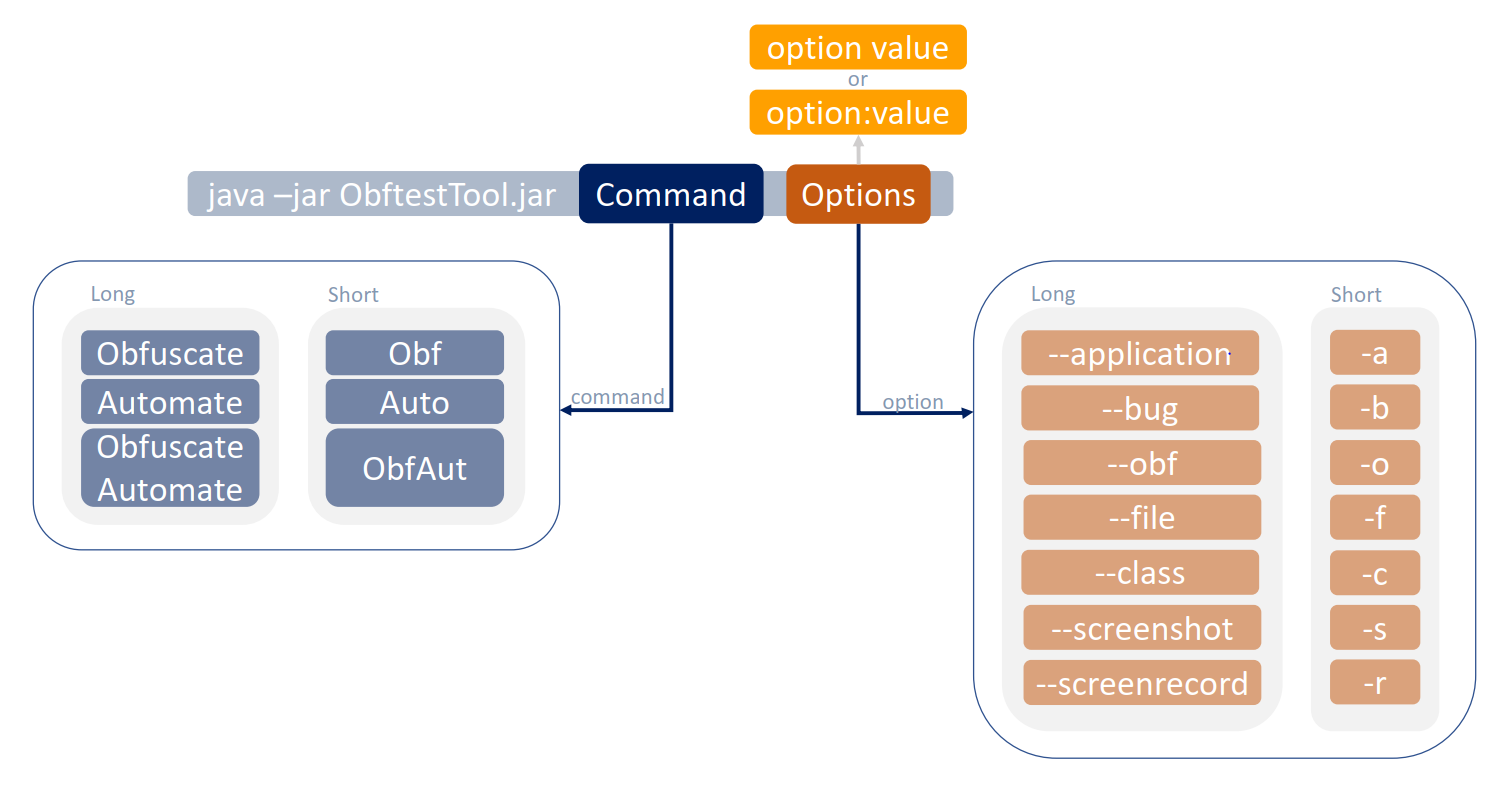
\includegraphics[scale=0.45]{cmd.string}
	\centering
	\caption{Struttura  stringa di lancio del tool}
    \label{fig:cmd.string}
\end{figure}
